% Title: gl2ps_renderer figure
% Creator: GL2PS 1.4.0, (C) 1999-2017 C. Geuzaine
% For: Octave
% CreationDate: Tue Oct 26 19:30:59 2021
\setlength{\unitlength}{1pt}
\begin{picture}(0,0)
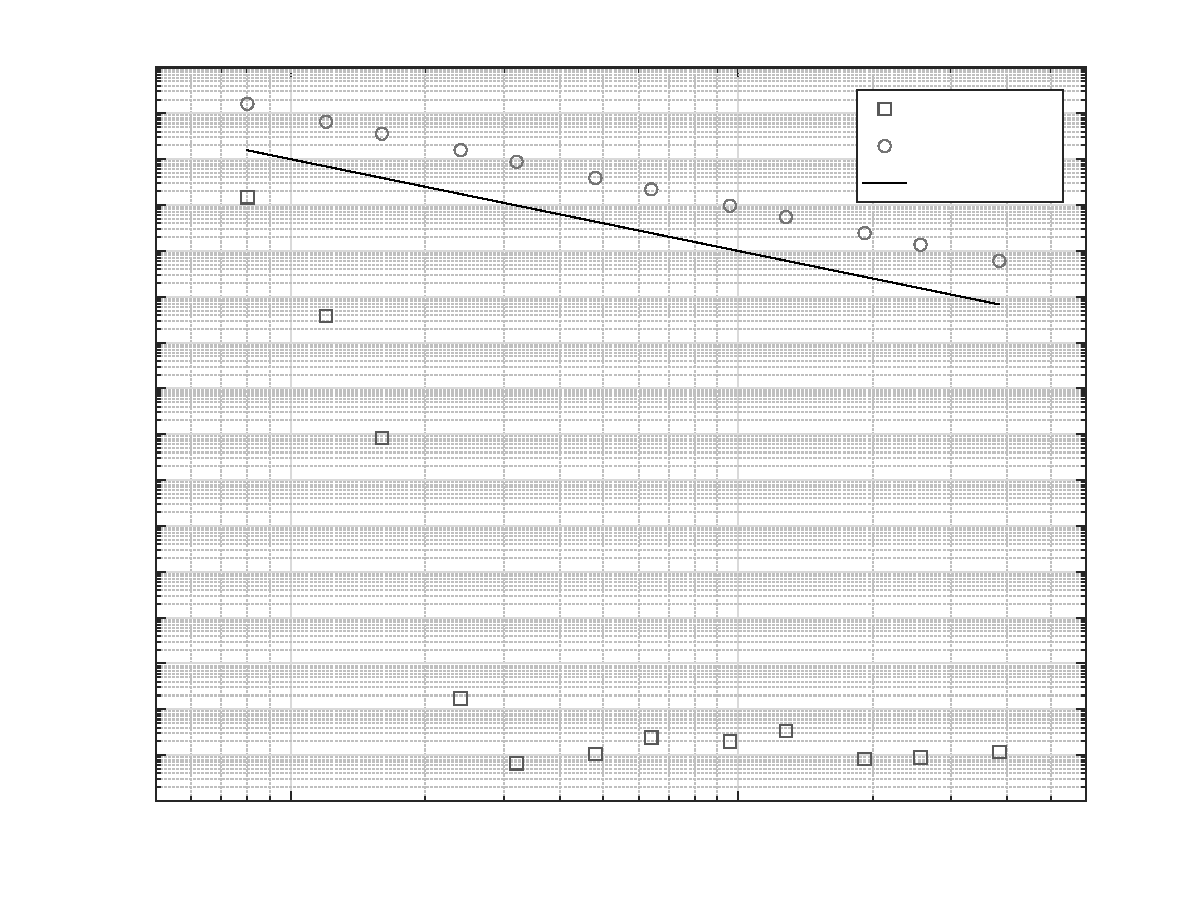
\includegraphics{figures/chap26/OUT/poisson_errorGray-inc}
\end{picture}%
\begin{picture}(576,432)(0,0)
\fontsize{10}{0}
\selectfont\put(139.511,40.0183){\makebox(0,0)[t]{\textcolor[rgb]{0.15,0.15,0.15}{{$10^{1}$}}}}
\fontsize{10}{0}
\selectfont\put(354.211,40.0183){\makebox(0,0)[t]{\textcolor[rgb]{0.15,0.15,0.15}{{$10^{2}$}}}}
\fontsize{10}{0}
\selectfont\put(69.8755,47.52){\makebox(0,0)[r]{\textcolor[rgb]{0.15,0.15,0.15}{{$10^{-16}$}}}}
\fontsize{10}{0}
\selectfont\put(69.8755,69.525){\makebox(0,0)[r]{\textcolor[rgb]{0.15,0.15,0.15}{{$10^{-15}$}}}}
\fontsize{10}{0}
\selectfont\put(69.8755,91.53){\makebox(0,0)[r]{\textcolor[rgb]{0.15,0.15,0.15}{{$10^{-14}$}}}}
\fontsize{10}{0}
\selectfont\put(69.8755,113.535){\makebox(0,0)[r]{\textcolor[rgb]{0.15,0.15,0.15}{{$10^{-13}$}}}}
\fontsize{10}{0}
\selectfont\put(69.8755,135.54){\makebox(0,0)[r]{\textcolor[rgb]{0.15,0.15,0.15}{{$10^{-12}$}}}}
\fontsize{10}{0}
\selectfont\put(69.8755,157.545){\makebox(0,0)[r]{\textcolor[rgb]{0.15,0.15,0.15}{{$10^{-11}$}}}}
\fontsize{10}{0}
\selectfont\put(69.8755,179.55){\makebox(0,0)[r]{\textcolor[rgb]{0.15,0.15,0.15}{{$10^{-10}$}}}}
\fontsize{10}{0}
\selectfont\put(69.8755,201.555){\makebox(0,0)[r]{\textcolor[rgb]{0.15,0.15,0.15}{{$10^{-09}$}}}}
\fontsize{10}{0}
\selectfont\put(69.8755,223.56){\makebox(0,0)[r]{\textcolor[rgb]{0.15,0.15,0.15}{{$10^{-08}$}}}}
\fontsize{10}{0}
\selectfont\put(69.8755,245.565){\makebox(0,0)[r]{\textcolor[rgb]{0.15,0.15,0.15}{{$10^{-07}$}}}}
\fontsize{10}{0}
\selectfont\put(69.8755,267.57){\makebox(0,0)[r]{\textcolor[rgb]{0.15,0.15,0.15}{{$10^{-06}$}}}}
\fontsize{10}{0}
\selectfont\put(69.8755,289.575){\makebox(0,0)[r]{\textcolor[rgb]{0.15,0.15,0.15}{{$10^{-05}$}}}}
\fontsize{10}{0}
\selectfont\put(69.8755,311.58){\makebox(0,0)[r]{\textcolor[rgb]{0.15,0.15,0.15}{{$10^{-04}$}}}}
\fontsize{10}{0}
\selectfont\put(69.8755,333.585){\makebox(0,0)[r]{\textcolor[rgb]{0.15,0.15,0.15}{{$10^{-03}$}}}}
\fontsize{10}{0}
\selectfont\put(69.8755,355.59){\makebox(0,0)[r]{\textcolor[rgb]{0.15,0.15,0.15}{{$10^{-02}$}}}}
\fontsize{10}{0}
\selectfont\put(69.8755,377.595){\makebox(0,0)[r]{\textcolor[rgb]{0.15,0.15,0.15}{{$10^{-01}$}}}}
\fontsize{10}{0}
\selectfont\put(69.8755,399.6){\makebox(0,0)[r]{\textcolor[rgb]{0.15,0.15,0.15}{{$10^{00}$}}}}
\fontsize{11}{0}
\selectfont\put(298.08,24.0183){\makebox(0,0)[t]{\textcolor[rgb]{0.15,0.15,0.15}{{grid size, $M$}}}}
\fontsize{11}{0}
\selectfont\put(14.8755,223.56){\rotatebox{90}{\makebox(0,0)[b]{\textcolor[rgb]{0.15,0.15,0.15}{{error}}}}}
\fontsize{11}{0}
\selectfont\put(298.08,409.6){\makebox(0,0)[b]{\textcolor[rgb]{0,0,0}{{Log--Log Plot of Pseudo-Spectral and Finite Difference Errors}}}}
\fontsize{9}{0}
\selectfont\put(438.176,379.696){\makebox(0,0)[l]{\textcolor[rgb]{0,0,0}{{pseudo--spectral}}}}
\fontsize{9}{0}
\selectfont\put(438.176,361.86){\makebox(0,0)[l]{\textcolor[rgb]{0,0,0}{{finite difference}}}}
\fontsize{9}{0}
\selectfont\put(438.176,344.025){\makebox(0,0)[l]{\textcolor[rgb]{0,0,0}{{$M^{-2}$}}}}
\end{picture}
